\titre{3}
\theme{trigo}
\auteur{Nathan Scheinmann}
\niveau{1M}
\source{sesamath-1M-trigo}
\type{serie}
\piments{2}
\pts{}
\annee{2425}

\contenu{
	\tcblower
Dans chaque cas, calculer la mesure de l'angle $\widehat{MNO}$; donner la valeur arrondie au degré.
\begin{tasks}(2)
	\task 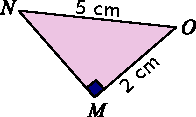
\includegraphics[scale=1]{../medias/1M/trigo/1M-exo-3-1}
	\task 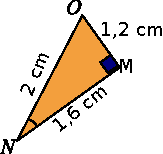
\includegraphics[scale=1]{../medias/1M/trigo/1M-exo-3-2}
	\task 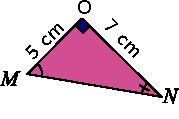
\includegraphics[scale=1]{../medias/1M/trigo/1M-exo-3-3}
	\task 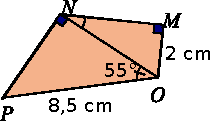
\includegraphics[scale=1]{../medias/1M/trigo/1M-exo-3-4}
\end{tasks}
}
\correction{

}

